\documentclass[11pt]{article}
\usepackage[top=1cm, bottom=2cm, left=1cm, right=1cm]{geometry}
\usepackage{ctex}
\usepackage{algorithm}
\usepackage{algorithmicx}
\usepackage{algpseudocode}
\usepackage{amsthm,amsmath,amssymb}
\usepackage[colorlinks=true,linkcolor=blue]{hyperref}
\usepackage{listings}
\usepackage{xcolor,xparse}
\usepackage{realboxes}
\usepackage{graphics}
\usepackage{graphicx}
\usepackage{mathrsfs}
\usepackage{wrapfig}
\usepackage{subfigure}
\usepackage{pifont}

\definecolor{cmdbg}{rgb}{0.9,0.9,0.9}
\lstset{%
	basicstyle=\ttfamily,
	breaklines = true,
	backgroundcolor=\color{cmdbg},
}
\DeclareDocumentCommand{\ccmd}{v}{% 参数 v 表示工作方法类似于 \verb
    \Colorbox{cmdbg}{\csname lstinline\endcsname!#1!}%
}

\makeatletter
\newenvironment{breakablealgorithm}
  {% \begin{breakablealgorithm}
   \begin{center}
     \refstepcounter{algorithm}% New algorithm
     \hrule height.8pt depth0pt \kern2pt% \@fs@pre for \@fs@ruled
     \renewcommand{\caption}[2][\relax]{% Make a new \caption
       {\raggedright\textbf{\ALG@name~\thealgorithm} ##2\par}%
       \ifx\relax##1\relax % #1 is \relax
         \addcontentsline{loa}{algorithm}{\protect\numberline{\thealgorithm}##2}%
       \else % #1 is not \relax
         \addcontentsline{loa}{algorithm}{\protect\numberline{\thealgorithm}##1}%
       \fi
       \kern2pt\hrule\kern2pt
     }
  }{% \end{breakablealgorithm}
     \kern2pt\hrule\relax% \@fs@post for \@fs@ruled
   \end{center}
  }
\makeatother

\author{李明钰 22307110156}
\title{计算物理作业n}

\begin{document}
\maketitle

\section{题目1:证明高斯消元法的时间复杂度为$O(N^3)$}
针对一个$n\times n$的矩阵
\begin{equation}
    A = \left[ 
    \begin{matrix}
a_{11} & a_{12} & \cdots & a_{1n} \\
a_{21} & a_{22} & \cdots & a_{2n} \\
\vdots  & \vdots  & \ddots & \vdots  \\
a_{n1} & a_{n2} & \cdots & a_{nn} \\
\end{matrix}
\right]
\end{equation}
根据高斯消元法(算法\ref{Gaussian Elimination Algorithm})将其变为上三角阵,
\begin{equation}
    A' = \left[ 
    \begin{matrix}
a_{11} & a_{12} & \cdots & a_{1n} \\
0 & a_{22} & \cdots & a_{2n} \\
\vdots  & \vdots  & \ddots & \vdots  \\
0 & 0 & \cdots & a_{nn} \\
\end{matrix}
\right]
\end{equation}
这对其中要进行消元的n列中的第p列,需要
\begin{itemize}
    \item 找到当前列的最大值,并将其所在行放在第$p$行,这需要时间$O(N)$
    \item 对第$q$行,$q=p+1,\ldots,n$需要进行如下操作
        \subitem 计算因子$f=\frac{a_{pq}}{a{pp}}$,这需要时间$O(1)$
        \subitem 更新第q行所有元素,这需要时间$O(N)$
    \item 对所有列重复这两步,这需要时间$O(N)$
\end{itemize}
综上,高斯消元法的总时间复杂度为$O(N^3)$

\subsection{伪代码}
如算法\ref{Gaussian Elimination Algorithm}所示
\begin{algorithm}
\caption{Gaussian Elimination Algorithm}
\label{Gaussian Elimination Algorithm}
\begin{algorithmic}[1]
\Procedure{GaussianElimination}{$A, b$}
    \State $n \gets \text{size of } A$
    \For{$p \gets 1 \textrm{ to } n-1$}
        \State Find the maximum element $A[i,p]$ in column $p$ below row $p$
        \State $maxRow \gets i$
        \If{$A[maxRow,p] = 0$}
            \State \textbf{continue}
        \EndIf
        \State Swap rows $p$ and $maxRow$ in $A$ and $b$
        \For{$i \gets p+1 \textrm{ to } n$}
            \State $f \gets \frac{A[i,p]}{A[p,p]}$
            \For{$j \gets p \textrm{ to } n$}
                \State $A[i,j] \gets A[i,j] - f \cdot A[p,j]$
            \EndFor
            \State $b[i] \gets b[i] - f \cdot b[p]$
        \EndFor
    \EndFor
    \State \textbf{return} BackwardSubstitution($A, b$)
\EndProcedure
\end{algorithmic}
\end{algorithm}

\section{题目2:用高斯消元法和partial-pivoting scheme求解方程组}
\subsection{题目描述}
用Gaussian elimination algorithm和partial-pivoting scheme求解方程组
\begin{equation}
    \begin{gathered}
2 x_{1}+3 x_{2}+5 x_{3}= \text{5} \\
3 x_{1}+4 x_{2}+8 x_{3}= \text{6} \\
  x_{1}+3  x_{2}+3  x_{3} = \text{5} 
\end{gathered}
\end{equation}
程序先将其改写为矩阵相乘的形式
\begin{equation}
    \mathbf{A}\vec{x} = \vec{b}
\end{equation}
其中,
\begin{equation}
    \mathbf{A} = \left[
\begin{matrix}
2 & 3 & 5 \\
3 & 4 & 8 \\
1 & 3 & 3 \\

\end{matrix}
\right] \qquad 
\vec{b} = (5,6,6)^{\text{T}}
\end{equation}
然后使用高斯消元法将扩展矩阵化为上三角阵,之后解出$\vec{x}=(2,2,-1)$,与理论解一致。
\subsection{伪代码}
如算法\ref{Gaussian Elimination Algorithm with Partial-pivoting Scheme}所示
\begin{algorithm}
\caption{Gaussian Elimination Algorithm with Partial-pivoting Scheme}
\label{Gaussian Elimination Algorithm with Partial-pivoting Scheme}}
\begin{algorithmic}[1]
\Procedure{GaussianElimination}{$A \in \mathbb{R}^{n \times n}, b \in \mathbb{R}^n$}
    \State $n \gets \text{size of } A$
    \For{$i \gets 0 \textrm{ to } n-2$}
        \State $p \gets i + \text{argmax}(A^T[i, i:])$ \Comment{Find the pivot index}
        \State $A_c \gets \text{copy}(A)$
        \State $b_c \gets \text{copy}(b)$
        \State $A[i] \gets A_c[p]$ \Comment{Swap the pivot row with the i-th row}
        \State $A[p] \gets A_c[i]$
        \State $b[i] \gets b_c[p]$
        \State $b[p] \gets b_c[i]$
        \For{$j \gets i+1 \textrm{ to } n-1$}
            \State $f \gets \frac{A[j][i]}{A[i][i]}$
            \State $A[j] \gets A[j] - f \cdot A[i]$
            \State $b[j] \gets b[j] - f \cdot b[i]$
        \EndFor
    \EndFor
    \State $x \gets \text{zeros}(n)$
    \For{$k \gets n-1 \textrm{ down to } 0$}
        \State $x[k] \gets \frac{b[k] - \text{dot}(A[k], x)}{A[k][k]}$
    \EndFor
    \State \Return $x$
    \EndProcedure
\end{algorithmic}
\end{algorithm}
\subsection{运行实例}
\begin{figure}[H]
    \centering
    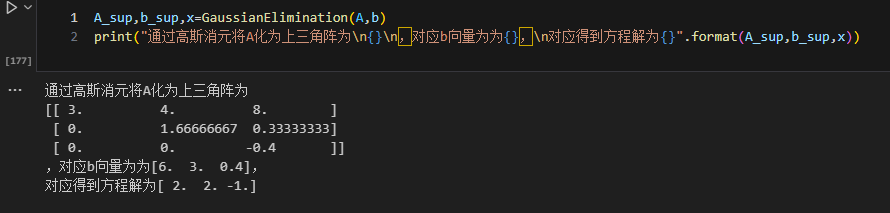
\includegraphics[width=\textwidth]{运行效果实例.png}
\end{figure}

\section{题目2:变分法解薛定谔方程}
\subsection{题目描述}
Solve the 1D Schrodinger equation with the potential (i) $V(x)=x^2$; (ii)$V(x)=x^4-x^2$ with the variational approach using a Gaussian basis (either fixed widths or fixed centers). Consider the three lowest energy eigenstates.
\subsection{程序描述}
对高斯基函数:
\begin{equation}
    \Phi_i(x)=(\frac{v_i}{\pi})^{1/2}e^{-v_i(x-s_i)^2}
\end{equation}
我们固定其方差不变,即限定所有$v_i$都等于1,只改变其$s_i$的值,根据公式
\begin{equation}
   S_{pk} = \int_{-\infty}^\infty\Phi_p^*(x)\Phi_k(x)dx
\end{equation}
和公式
\begin{equation}
    H_{pk}=\int_{-\infty}^{\infty}\Phi_{p}^{*}(x)H\Phi_{k}(x)dx
\end{equation}
借助Mathematica计算(文件夹中 积分运算.nb)出$H_{pk}$与$v_p,v_k$的解析关系,为再在$(-200,200)$之间均匀取n个值,作为基函数中心$s_i$的取值,计算出相应具体的矩阵$S$和$H$。
再求解广义特征值问题
\begin{equation}
    HC =ESC
\end{equation}
即可得到本征值和高斯基下的对应的本征矢。

\subsection{输出实例}
\subsubsection{不同基数量下的本征值}
模拟计算出的$V=x^2$下的最低的三个能量本征值与选取基函数数量本征值对应关系如表\ref{本征值与基函数数量对应关系}所示

\begin{table}[!ht]
\label{本征值与基函数数量对应关系}
    \centering
    \begin{tabular}{|l|l|l|l|}
    \hline
        \textbf{基数量n} & \textbf{E1} & \textbf{E2} & \textbf{E3} \\ \hline
        50 & 17.90972511 & 17.90972511 & 151.18752603 \\ \hline
        100 &  5.32539866 & 5.33703698 & 37.98094899 \\ \hline
        200 & 1.66828647 & 3.02394632 & 10.48343753 \\ \hline
        300 & 1.04669018  & 3.04764203  & 5.97892026 \\ \hline
        400 & 1.00101988  & 3.0040235   & 5.07659885 \\ \hline
        500 & 1.00000583  & 3.00005203  & 5.00137461 \\ \hline
        600 & 1.00000001 & 3.00000015 & 5.00000512 \\ \hline
    \end{tabular}
\end{table}
\subsection{运行实例}
设定$n=600$计算得到最低三个能级的本征值如图\ref{fig:输出最低三个能级本征值}所示,画出相应的本征态如图\ref{fig:V1最低三个能级对应本征态函数}\ref{fig:V2最低三个能级对应本征态函数}所示
\begin{figure}
    \centering
    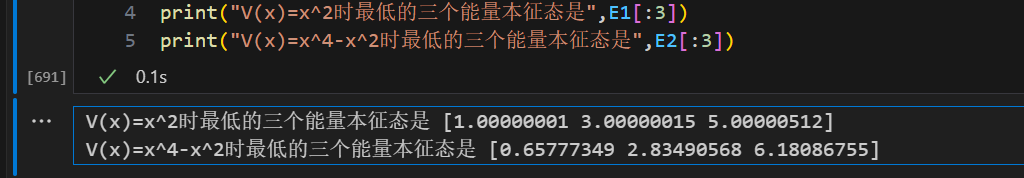
\includegraphics[width=0.5\linewidth]{T3输出实例.png}
    \caption{输出最低三个能级本征值}
    \label{fig:输出最低三个能级本征值}
\end{figure}
\begin{figure}
    \centering
    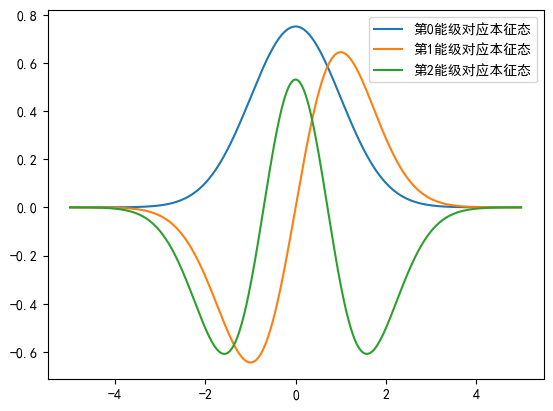
\includegraphics[width=0.5\linewidth]{V1本征态.png}
    \caption{$V=x^2$最低三个能级对应本征态函数}
    \label{fig:V1最低三个能级对应本征态函数}
\end{figure}
\begin{figure}
    \centering
    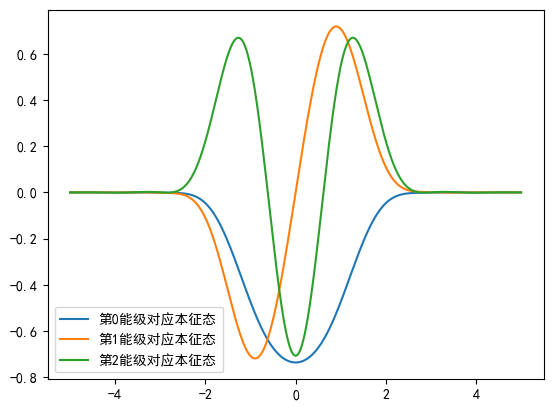
\includegraphics[width=0.5\linewidth]{V2本征态.png}
    \caption{$V=x^4-x^2$最低三个能级对应本征态函数}
    \label{fig:V2最低三个能级对应本征态函数}
\end{figure}

\subsection{伪代码}
\begin{breakablealgorithm}
\begin{algorithmic}
    

\caption{Gaussian Basis Function and Matrix Calculation}
\Require{$x$, $s$, $v$ (for Gaussian basis), $v_i$, $v_j$, $s_i$, $s_j$ (for H and S matrices)}
\KwOut{$S$, $H_1$, $H_2$, $E_1$, $E_2$, $C_1$, $C_2$}

\SetKwFunction{GaussianBasisFunc}{GaussianBasisFunc}
\SetKwFunction{CalculateS}{Calculate\_S}
\SetKwFunction{CalculateH1}{Calculate\_H1}
\SetKwFunction{CalculateH2}{Calculate\_H2}

\BlankLine
\textbf{Define GaussianBasisFunc}($x, s, v$): \\
\Indp
    \textbf{return} $\sqrt{\frac{v}{\pi}} \exp(-v (x - s)^2)$
\Indm

\BlankLine
\textbf{Define Calculate\_S}($v_i, v_j, s_i, s_j$): \\
\Indp
    $\text{exponent} \gets - \frac{v_i v_j (s_i - s_j)^2}{v_i + v_j}$ \\
    \textbf{return} $\frac{\sqrt{v_i} \sqrt{v_j} \exp(\text{exponent})}{\sqrt{\pi} \sqrt{v_i + v_j}}$
\Indm

\BlankLine
\textbf{Define Calculate\_H1}($v_i, v_j, s_i, s_j$): \\
\Indp
    $\text{part1} \gets \frac{1}{2 \sqrt{\pi} (v_i + v_j)^{5/2}}$ \\
    $\text{exponent} \gets -\frac{(s_i - s_j)^2 v_i v_j}{v_i + v_j}$ \\
    $\text{part2} \gets \exp(\text{exponent})$ \\
    $\text{part3} \gets \sqrt{v_i} \sqrt{v_j}$ \\
    $\text{part4} \gets v_i + v_j + 2 s_j^2 v_j^2 + 4 v_i v_j (s_i s_j + v_j) + 2 v_i^2 (s_i^2 + 2 v_j - 4 (s_i - s_j)^2 v_j^2)$ \\
    $H_1 \gets \text{part1} \times \text{part2} \times \text{part3} \times \text{part4}$ \\
    \textbf{return} $H_1$
\Indm

\BlankLine
\textbf{Define Calculate\_H2}($v_i, v_j, s_i, s_j$): \\
\Indp
    $\text{term1} \gets \frac{1}{4 \sqrt{\pi} (v_i + v_j)^{9/2}} \sqrt{v_i} \sqrt{v_j}$ \\
    $\text{exp\_part} \gets \exp(-\frac{(s_i - s_j)^2 v_i v_j}{v_i + v_j})$ \\
    $\text{term2\_vi2} \gets v_i^2 (3 - 2 v_i + 4 s_i^2 v_i (3 + (-1 + s_i^2) v_i))$ \\
    $\text{term2\_vi\_vj} \gets 2 v_i (3 + v_i (-3 + s_i^2 (6 - 4 v_i) - 4 s_i s_j (-3 + v_i) + 8 s_i^3 s_j v_i)) v_j$ \\
    $\text{term2\_vj2} \gets (3 + 2 v_i (-3 + 4 s_i s_j (3 - 2 v_i) - 2 s_j^2 (-3 + v_i) + 2 s_i^2 (-1 + 6 s_j^2) v_i)) v_j^2$ \\
    $\text{term2\_vj3} \gets 2 (-1 + 2 s_j (-2 s_i v_i + s_j (3 + (-2 + 4 s_i s_j) v_i))) v_j^3$ \\
    $\text{term2\_vj4} \gets 4 s_j^2 (-1 + s_j^2) v_j^4$ \\
    $\text{correction\_term} \gets -8 v_i v_j (v_i + v_j)^2 (-v_j + v_i (-1 + 2 (s_i - s_j)^2 v_j))$ \\
    $\text{term2} \gets \text{term2\_vi2} + \text{term2\_vi\_vj} + \text{term2\_vj2} + \text{term2\_vj3} + \text{term2\_vj4} + \text{correction\_term}$ \\
    $H_2 \gets \text{term1} \times \text{exp\_part} \times \text{term2}$ \\
    \textbf{return} $H_2$
\Indm

\BlankLine
\textbf{Define Constants:}\\
\Indp
$n\_basis \gets 600$ \quad \text{(number of basis functions)} \\
$v \gets 1$ \quad \text{(constant width of basis functions)} \\
$n\_x \gets 600$ \quad \text{(number of points for plotting)} \\
$s\_max \gets 200$ \quad \text{(maximum value of basis function centers)} \\
$x\_max \gets 5$ \\
$s\_min \gets -s\_max$ \\
$s\_array \gets \text{linspace}(s\_min, s\_max, n\_basis)$
\Indm

\BlankLine
\textbf{Initialize Matrices:} \\
\Indp
$H_1 \gets \mathbf{0}_{n\_basis \times n\_basis}$ \\
$H_2 \gets \mathbf{0}_{n\_basis \times n\_basis}$ \\
$S \gets \mathbf{0}_{n\_basis \times n\_basis}$
\Indm

\BlankLine
\textbf{Calculate H and S Matrices:}\\
\For{$i \gets 0$ \textbf{to} $n\_basis - 1$}{
    \For{$j \gets 0$ \textbf{to} $n\_basis - 1$}{
        $H_1[i][j] \gets \text{Calculate\_H1}(v, v, s\_array[i], s\_array[j])$ \\
        $H_2[i][j] \gets \text{Calculate\_H2}(v, v, s\_array[i], s\_array[j])$ \\
        $S[i][j] \gets \text{Calculate\_S}(v, v, s\_array[i], s\_array[j])$
    }
}

\BlankLine
\textbf{Compute Eigenvalues and Eigenvectors:}\\
$E_1, C_1 \gets \text{eigh}(H_1, S)$ \\
$E_2, C_2 \gets \text{eigh}(H_2, S)$

\BlankLine
\textbf{Print Results:} \\
\Indp
\textbf{print} "Lowest three energy eigenstates for $V(x) = x^2$: $E_1[:3]$" \\
\textbf{print} "Lowest three energy eigenstates for $V(x) = x^4 - x^2$: $E_2[:3]$"
\Indm

\end{algorithmic}
\end{breakablealgorithm}[H]


\end{document}
